%%%%%%%%%%%%%%%%%%%%%%%%%%%%%%%%%%%%%%%%%%%%%%%%%%%%%%%%%%%%%%%%%%%%%%%%%%%%%%%%%%%%%%%%%%%%%%%%%%%%%%%%%%%%%%%%
%%%%%%%%%%%%%%%%%%%%%%%%%%%%%%%%%%%%%%%%%%%%%%%%%%%%%%%%%%%%%%%%%%%%%%%%%%%%%%%%%%%%%%%%%%%%%%%%%%%%%%%%%%%%%%%%
%%%%%                                          ELEKTROSTATIK                                           %%%%%%%%%
%%%%%%%%%%%%%%%%%%%%%%%%%%%%%%%%%%%%%%%%%%%%%%%%%%%%%%%%%%%%%%%%%%%%%%%%%%%%%%%%%%%%%%%%%%%%%%%%%%%%%%%%%%%%%%%%
%%%%%%%%%%%%%%%%%%%%%%%%%%%%%%%%%%%%%%%%%%%%%%%%%%%%%%%%%%%%%%%%%%%%%%%%%%%%%%%%%%%%%%%%%%%%%%%%%%%%%%%%%%%%%%%%
\setlength{\parindent}{0pt} % kein einrücken der listen
\renewcommand{\arraystretch}{1.3}
\skriptsection{Elektrostatik}{3-1}
 

\renewcommand{\arraystretch}{1.8}
\begin{tabular}[c]{ | p{4.5cm} | p{9cm} | p{4cm} | }
	\hline
	\textbf{Name}
	& \hspace{-6pt}\begin{tabular}[t]{p{2.75cm} | p{2.75cm} | p{2.7cm}}
			\textbf{Allg.} 
			& \textbf{Pt.-Q}
			& \textbf{Homogen}
			\\
		 \end{tabular} 
	& \textbf{Info}\\ 
	\hline

Dielektrizitätskonstante
	& $\varepsilon_0 =  8.8542 \cdot 10^{-12} \frac{As}{Vm}$ 
	& \\
	\hline

Elementarladung
	& $e = 1.602 \cdot 10^{-19} C$
	& \\
	\hline
	\hline

Coulombsches Gesetz $^{1)}$
	& \hspace{-6pt}\begin{tabular}[t]{p{2.75cm} | p{2.75cm} | p{2.7cm}}
			$\vec{F} = \vec{E}\cdot Q $
			& $F = \frac{Q_1}{4 \pi \varepsilon r^2} \cdot Q_2$
			& 
			\\
		 \end{tabular} 
	& ($F>0 \rightarrow$ Abstossung) \\
	\hline

Elektrische Feldstärke $^{2,7)}$
	&\hspace{-6pt}\begin{tabular}[t]{p{2.75cm} | p{2.75cm} | p{2.7cm}}
			$\vec{E} = \frac{\vec{F}}{Q} $
			& $E = \frac{Q}{4\pi\varepsilon r^2}$ 
			& $ E = \frac{U}{d} $\\
			& $ E(r) = \frac{E_{R_1} \cdot {R_1}^2}{r^2}$&\\
		 \end{tabular} 
	& $[E] = \frac{V}{m}$ \\
	\hline

Arbeit
	& \hspace{-6pt}\begin{tabular}[t]{p{2.75cm} | p{2.75cm} | p{2.7cm}}
			$W_{AB} = \int \limits^b_a F(r) dr$
			& $ = \frac{Q_1 \cdot Q_2}{4 \pi \varepsilon
				}(\frac{1}{a} - \frac{1}{b})$
			& $= U_{AB} \cdot Q \ ^{3)}$ \\
		 \end{tabular}   
	& $[W] = Ws = J; [p] = W$ \\
	\hline

Spannung innerh. E-Feld $^{4)}$
	& \hspace{-6pt}\begin{tabular}[t]{p{2.75cm} | p{2.75cm} | p{2.7cm}}
			$U_{AB} = \int\limits_A^B \vec{E}(s) d\vec{s}$
			& $ = \varphi_A - \varphi_B$ 
			& $ = \frac{W_{AB}}{Q} = \vec{E} \cdot \vec{l}_{AB}$
			\\
		 \end{tabular} 
	& \\
	\hline

Potential $^{5)}$
	& \hspace{-6pt}\begin{tabular}[t]{p{2.75cm} | p{2.75cm} | p{2.7cm}}
			$\varphi = \frac{W}{Q} = \sum\limits^n_{i=1} \varphi_{_{Q_i}}$
			& $\varphi = \frac{Q_1}{4 \pi \varepsilon r}$
			& \\
			$= \frac{aufgew. Arbeit}{herangesch. Q}$
			& $\varphi = \frac{1}{4 \pi \varepsilon} \sum\limits_{i=1}^n \frac{Q_i}{r_i}$&\\
		 \end{tabular} 
	& $[\varphi] = V = \frac{Ws}{As} = \frac{VAs}{As}$ \\
	\hline
	\hline

Elektrische Flussdichte $^{6)}$
	& \hspace{-6pt}\begin{tabular}[t]{p{2.75cm} | p{2.75cm} | p{2.7cm}}
			$\vec{D} = \varepsilon \cdot  \vec{E} $
			& $D = \frac{Q}{4\pi r^2}$
			& $D = \frac{\Psi}{A\cos \varphi}$
			\\
		 \end{tabular} 
	& $[D] = \frac{C}{m^2} = \frac{As}{m^2}$ \\
	\hline

Elektrischer Fluss
	& \hspace{-6pt}\begin{tabular}[t]{p{2.75cm} | p{2.75cm} | p{2.7cm}}
			$\Psi = \int\limits_A \vec{D} \cdot d \vec{A}$
			& 
			& $\Psi = D \cdot A \cdot \cos \varphi$
			\\
		 \end{tabular} 
	& $[\Psi] = As, C$ \\
	\hline

Gauss'scher Satz (El-Statik) 
	& $ \Psi_{Huelle} = \sum Q_{eingeschlossen} $ 
	& \\
	\hline
	\hline

Kapazität
	& $C = \frac{Q}{U}$
	& $[C] = F = \frac{C}{V} = \frac{As}{V}$ \\
	\hline

Flächenladungsdichte
	& $\sigma = \frac{Q}{A} \rightarrow$ besteht an Grenzfläche zwischen Leiter \& Isolator
	& $ [\sigma] = \frac{C}{m^2} $\\
	\hline

Ladung
	& $Q = I \cdot t = C \cdot U$
	& $[Q] = As = C$ \\
	\hline

Energiedichte
 	& $w=\frac{W}{V} = \frac{1}{2} \varepsilon \cdot E^2 = \frac{1}{2}D\cdot E = \frac{D^2}{2\cdot \varepsilon}$
 	& $[w]=\frac{J}{m^3}$ \\ 
	\hline

Stromstärke    
  	 & $ I =  \frac{Q}{t} = \frac{\Delta Q}{\Delta t}  \qquad i = \frac{dQ}{dt}  $
	 &  $[I]=\frac{As}{s} = A$\\
	\hline

\end{tabular}
\renewcommand{\arraystretch}{1}

\subsection{Anmerkungen zu den Formeln}
	\textbf{1)} Gilt nur für Punktladungen exakt; für geladene Körper nur wenn 
		Körperabmessung $\ll$ Abstand \\
	\textbf{2)} $Q > 0$: $\vec{E}$ gleiche Richtung wie $\vec{e}_r$ $\leftrightarrow$ $Q < 0$: 
		$\vec{E}$ entgegengesetzte Richtung wie $\vec{e}_r$.
		Der Radius wird immer von der Kugelmitte aus genommen (d.h. an einer
		Kugeloberfläche besteht eine Feldstärke!)\\
	\textbf{3)} Wird eine Ladung von A nach B verschoben, so hängt die aufzubringende bzw. 
		abgeg. Energie \textit{nicht vom Verschiebungsweg}, sondern nur von der 
		Potentialdifferenz $\varphi_B - \varphi_A = U_{AB}$ab.\\
	\textbf{4)} Weg AB so wählen, dass $\vec{E} \perp \vec{s}$ oder $\vec{E} \parallel \vec{s}$ 
		\\
	\textbf{5)} Potential nimmt in Feldlinienrichtung ab.\\
	\textbf{6)} Im Leiter existiert kein E-Feld $\Rightarrow D = 0$! $\rightarrow$ D ist 
		materialunabhängig.

\begin{tabular}[t]{ll}
	\parbox{6cm}{\textbf{7)} Superposition durch Vektoraddition\\
	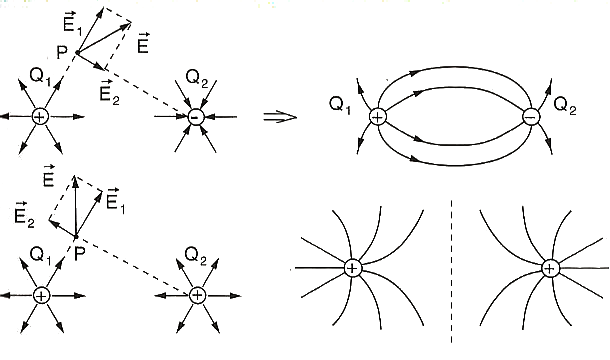
\includegraphics[width=6cm]{./bilder/e-feldlinien.png}
	}
	& \parbox{12cm}{
	\skriptsubsection{Leiter im Feld}{1-18}
	\itemize {
		\item Innere des Leiters ist feld- (Influenz) und ladungsfrei (Faradayscher Käfig)
		\item Feldlinien stehen senkrecht zur Leiteroberfläche
		\item Oberfläche des Leiters ist äquipotential
	}\\
	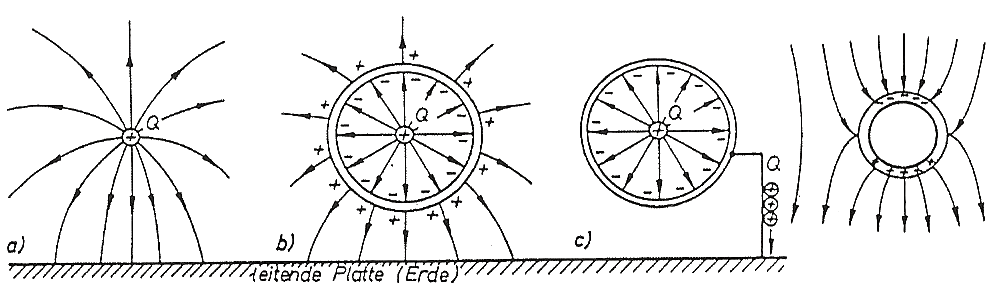
\includegraphics[width=7cm]{./bilder/leiter-im-efeld.png}}
\end{tabular}

\skriptsubsection{Kondensator, Kapazität}{3-24}
	\paragraph{Kapazitätsberechnung} $\Psi_{Huelle} = D \cdot A = Q \Rightarrow D(r) = 	
	\frac{Q}{A(r)} \Rightarrow E(r) = \frac{D(r)}{\epsilon}\Rightarrow U = \int E(r) \cdot dr 
	\Rightarrow C = \frac{Q}{U}$\\

\renewcommand{\arraystretch}{2}
\begin{tabular}{p{5cm} p{3cm} p{5cm} p{5cm}}
Plattenkondensator
	& $\displaystyle C = \frac{\varepsilon A}{d}$
	& Koaxialkabel (Zyl.) $(r_a > r_i)$
	& $\displaystyle C = \frac{2 \pi \varepsilon l}{\ln \frac{r_a}{r_i}} $ \\
Kugelkondensator $(R_2 > R_1)$
	& $\displaystyle C = 4 \pi \varepsilon \frac{R_1 R_2}{R_2 - R_1}$ 
	& Doppelleitung
	& $\displaystyle C = \frac{\pi \varepsilon l}{\ln \frac{a-r}{r}} \approx 
\frac{\pi \varepsilon l}{\ln \frac{a}{r}} (l \gg a \gg r)$
\end{tabular} 
\renewcommand{\arraystretch}{1}  
\vspace{0.2cm} \\ 

\parbox[t]{4.5cm}{\textbf{Koaxialkabel} \\ \vspace{.2cm} \\ 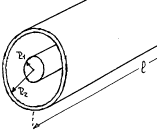
\includegraphics[width=4cm]
	{./bilder/e-c-koaxialkabel.png}}
\parbox[t]{4.5cm}{\textbf{Doppelleitung} \\ \vspace{.2cm} \\ 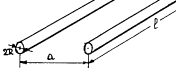
\includegraphics[width=4cm]
	{./bilder/e-c-paralleldraht.png}}
\parbox[t]{10cm}{\textbf{Spezielle elektrische Felder} \\ 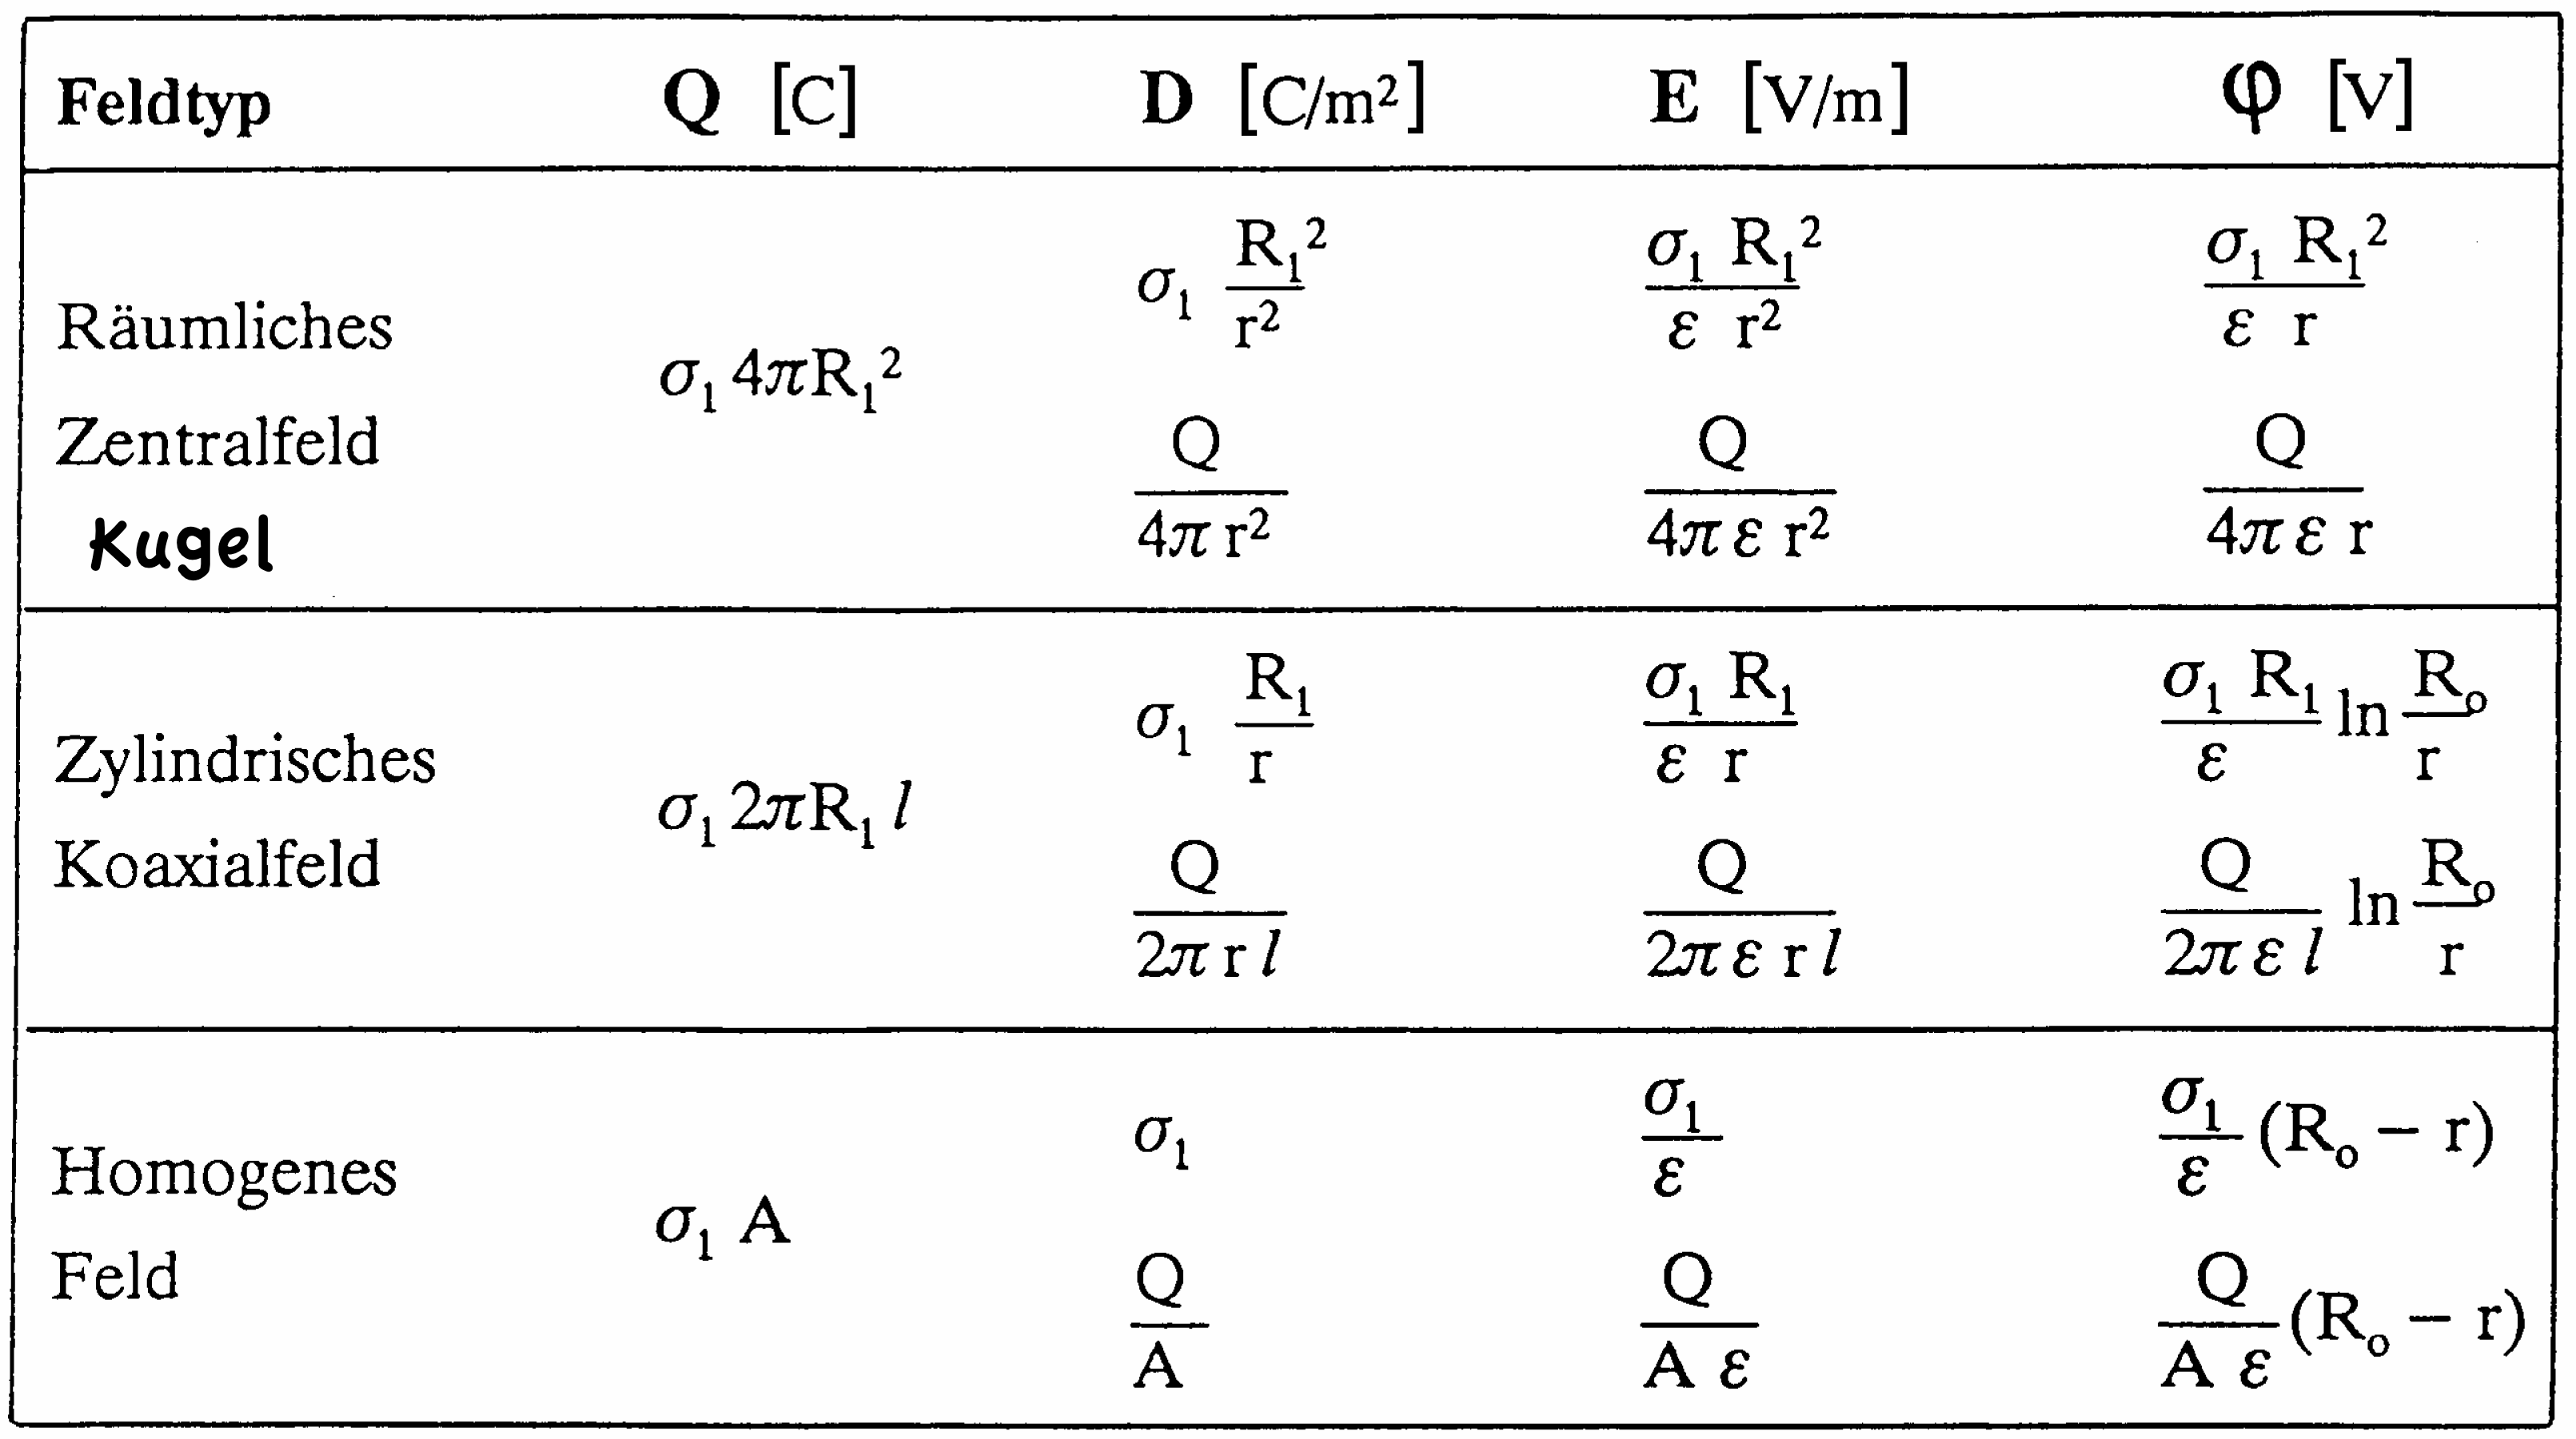
\includegraphics[width=8cm]	
	{./bilder/e-c-speziellefelder.png} \\
	$\sigma = \frac{Q}{A}; R_0 =$ Abstand zum Bezugspunkt; $r =$ Abstand zur Ladung}


\skriptsubsection{Schaltungen mit Kapazitäten}{3-30}
Kapazitäten werden in den Grundschaltungen genau \textbf{verkehrt gegenüber Widerständen} berechnet.\\
\begin{tabular}{llll}
Parallelschaltung zweier C
	& $C_{tot} = C_1 + C_2 \qquad \qquad $ 
	& Parallelschaltung mehrerer C 
	& $C_{tot} = \sum\limits_{n=1}^\infty C_n \rightarrow$ alle gleiche U 	\\
Serieschaltung zweier C
	& $C_{tot} = \frac{C_1 C_2}{C_1 + C_2}$
	& Serieschaltung mehrerer C
	& $\frac{1}{C_{tot}} = \sum\limits^n_{k=1} \frac{1}{Q_k} \rightarrow$ alle gleiche Q 
\end{tabular}


\skriptsubsection{Polarisation und Dielektrika}{3-31}
Man unterscheidet zwischen zwei verschiedenen Dielektrika:
\begin{itemize}
	\item Die \textbf{dipolfreien} Moleküle \textbf{unpolarer Dielektrika} werden durch die wirkung des elektrischen Feldes verzerrt. \\
	Man nennt dies eine \textbf{Verschiebungspolarisation}.
	\item Bei \textbf{polaren Dielektrika} (z.B. $H_2O$) haben die Moleküle ohne äussere Einwirkung bereits Dipolcharakter. \\
	Es entsteht nebst der Verschiebungspolarisation noch eine \textbf{Orientierungspolarisation}.
\end{itemize}
%Bei Plattenkondensatoren mit verschiedenen Dielektrizitätsconstanten: 

\parbox[t]{10.5cm} {
	\subsubsection{Querschichtung}
	\parbox[h]{6cm}{
		$$D = \frac{Q}{A} \Rightarrow \text{konstant}$$ 
		$$E_1 = \frac{D}{\epsilon_1}  = \frac{U}{d_1 + \frac{\epsilon_1}{\epsilon_2} \cdot d_2}; E_2 = \frac{D}{\epsilon_2}$$
		$$U = E_1 d_1 + E_2 d_2 \Rightarrow D = \frac{U}{\frac{d_1}{\epsilon_1} + \frac{d_1}		
			{\epsilon_2}}$$
		$$\frac{E_1}{E_2} = \frac{\epsilon_2}{\epsilon_1}$$
	}
	\parbox[h]{4cm}{
		\includegraphics[width=3cm]{./bilder/schichtung_quer.png}
	}
}
\parbox[t]{10cm} {
	\subsubsection{Längsschichtung}
	\parbox[h]{5cm}{
		$$E = \frac{U}{d} \Rightarrow \text{konstant}$$
		$$D_1 = E \cdot {\epsilon_1} ; D_2 = E \cdot {\epsilon_2}$$
		$$\epsilon_2 > \epsilon_1 \Rightarrow D_2 > D_1$$
		$$\frac{D_2}{D_1} = \frac{\epsilon_2}{\epsilon_1}$$
	}
	\parbox[h]{4cm}{
		\includegraphics[width=3cm]{./bilder/schichtung_laengs.png}
	}
}

\parbox[t]{8.7cm} {
	\subsubsection{Feldlinien an Grenzfl. ver. Dielektrika}
	\parbox{4.5cm}{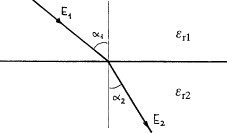
\includegraphics[width=4cm]{./bilder/e-grenzflaechen-dielektrika.png}}
	\parbox{3.5cm}{
	$$ \frac{\tan(\alpha_1)}{\tan(\alpha_2)} = \frac{\varepsilon_{r1}}{\varepsilon_{r2}} $$ }
}
\parbox[t]{9.4cm}{
\subsubsection{Eigenschaften von Dielektrika}
	\tabcolsep0pt
	\begin{tabular}[t]{p{5.2cm} p{4.8cm}}
		homogen: $\varepsilon_r$ ist ortsunabhängig 
			& inhomogen: $\varepsilon_r$ ist ortsabhängig \\
		linear: $\varepsilon_r$ ist feldstärkeunabh. 
			& nichtlinear: $\varepsilon_r$ ist feldstärkeabh. \\ 
		isotrop: $\varepsilon_r$ ist richtungsunabh. 
			& anisotrop: $\varepsilon_r$ ist richtungsabh. 
	\end{tabular}
} 

\subsubsection{Relative Dielektrizitätskonstanten $\varepsilon_r$ verschiedener Stoffe bei $ 20^\circ C $ }
\begin{tabular}[c]{ p{2cm}  p{1.7cm}  p{2.5cm}  p{1.7cm} p{2cm}  p{1.7cm} p{2cm}  p{1.7cm} }
Azeton & 21.5
& Bernstein & 2.8
& Diamant & 16.5
& Glas & 5 \ldots 7 \\
Glimmer & 5 \ldots 8
& Gummi & 2.7
& Hartpapier & 5 \ldots 6
& Harzöl & 2 \\
Mineralöl  & 2.2
& Pertinax  & 4.8
& Petroleum & 2.1
& Polystyrol & 2.6 \\
Quarz & 3.8 \ldots 5
& Keram. Stoffe  & 10 \ldots 1000
& Vakuum & 1
& Wasser & 80.3

\end{tabular}

\skriptsubsection{Energie und Kraft im elektrostatischen Feld}{3-33}
Im Kondensator gespeicherte Energie: $\qquad\boxed{W = \underbrace{\frac{1}{2} \cdot C \cdot U^2}_{U = konst} = \frac{1}{2} \cdot Q \cdot U = \underbrace{\frac{1}{2} \cdot \frac{Q^2}{C}}_{Q = konst} }$\\

\parbox{5cm}{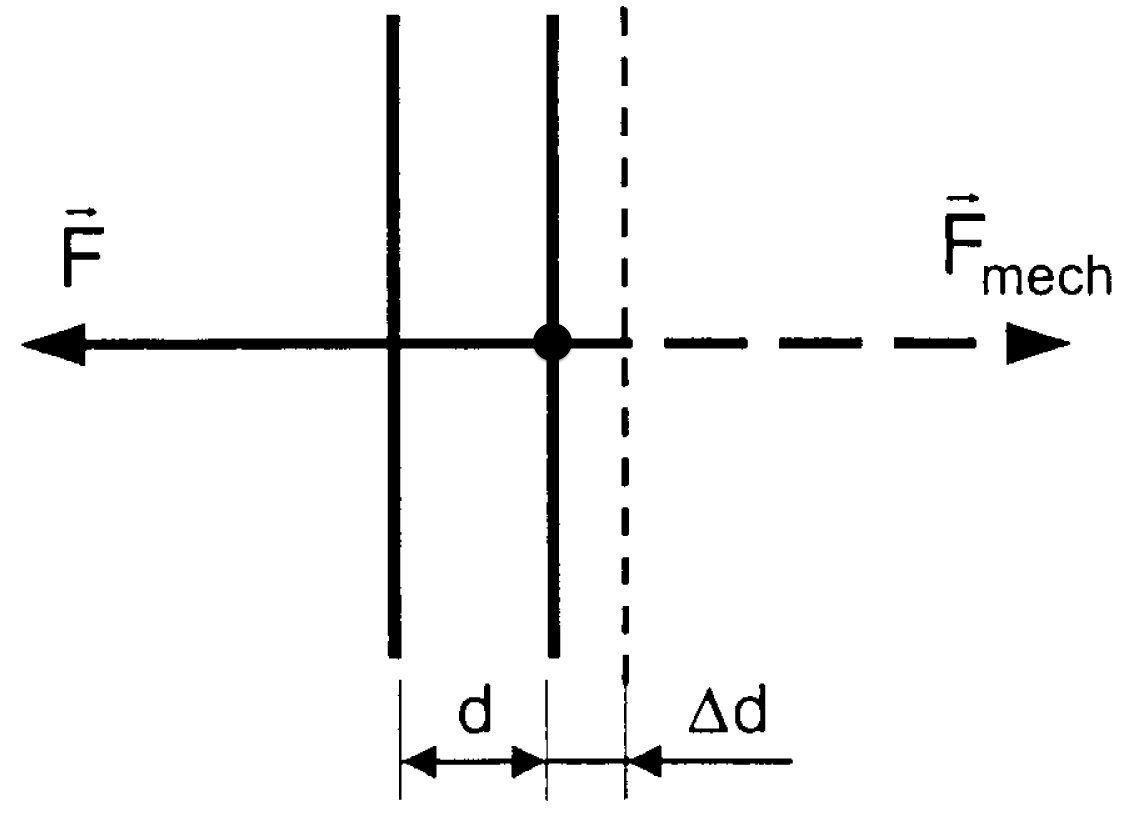
\includegraphics[width=4cm]{./bilder/e-c-kraft.png}}
\parbox{13cm}{
	Grundsätzlich versuchen sich die Feldlinien zu verkürzen $\rightarrow$ Die Kraft auf die 	
	Grenzflächen ist so gerichtet, dass sie die Kapazität zu vergrössern sucht. \\	
	Die Kraft berechnet sich mittels dem \textbf{Prinzip der virtuellen Verschiebung}. \\ \\
	$\qquad F = F_{mech} = \left| \frac{\mathrm dW}{\mathrm dd} \right| \qquad$ 
	$\mathrm dW = \frac{1}{2} \varepsilon \cdot E^2 \cdot A \cdot \mathrm dd \quad 
	\Rightarrow \quad \boxed{ F = \frac{1}{2} 
	\varepsilon \cdot E^2 \cdot A = \frac{1}{2} \varepsilon \cdot \frac{U^2}{d^2} \cdot A}$ \\
	$$ F = \frac{1}{2} \cdot U^2 \cdot \frac{\mathrm dC}{\mathrm dd}, \text{ (für U = const.)} 
	\qquad \text{ oder } \qquad 
	F = \frac{1}{2} \cdot Q^2 \cdot \frac{\mathrm d}{\mathrm dd} \left( \frac{1}{C} \right), 	
	\text{ (für Q = const.)}$$
	\\ 
	Formeln für $F$ gelten auch, wenn C an Quelle angeschlossen ist, dafür muss jedoch $|F|$		
	genommen werden.} 


\skriptsubsection{Teilkapazitäten, Mehrleitersysteme}{3-36}
Um die kapazitive Beziehung von mehrehren gegeneinander isolierten Leitern (sog. Mehrleitersystem) zu bestimmen kann man deren 
Teilkapazitäten berechnen. So lassen sich z.B. die Teilkapazitäten eines mehradrigen Kabels berechnen. \\

\parbox{5cm}{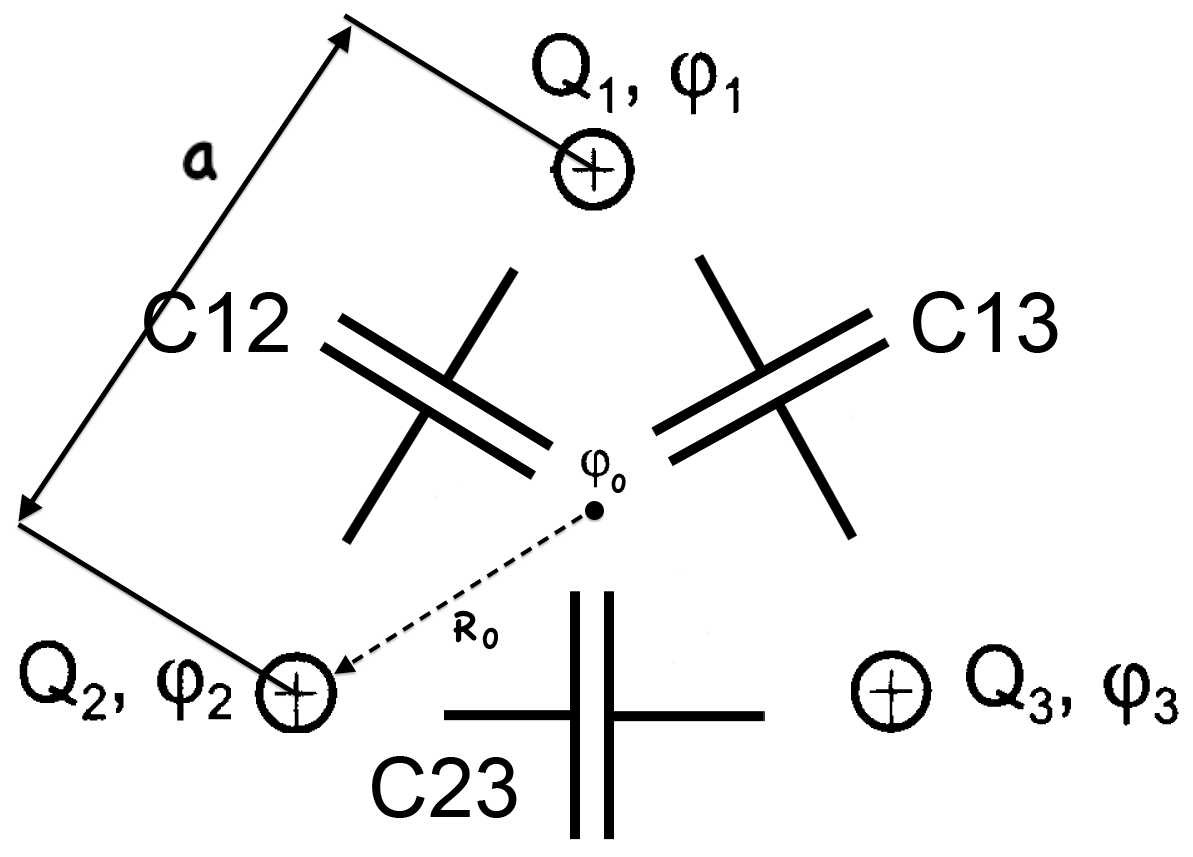
\includegraphics[width=4cm]{./bilder/e-c-teilkapazitaeten.png}}
\parbox{13cm}{
	Zur Berechnung der Teilkapazitäten geht man wie folgt vor:
	\begin{enumerate}
    	\item Ladungen $Q_1, Q_2, Q_3$ (mit $Q_1 + Q_2 + Q_3 = 0$) als gegeben betrachten 	
		und $\varphi_1, \varphi_2, \varphi_3$ in Bezug zur Mitte berechnen.\\ Bsp $\varphi_1 
		= \frac{1}{2\cdot \pi \cdot \epsilon\cdot l}(Q_1 \cdot \ln{\frac{R_0}{R}}+Q_2 \cdot \ln{\frac{R_0}{a}}+Q_3 
		\cdot \ln{\frac{R_0}{a}})$
    	\item $U_{12}, U_{23}, U_{13}$ aus $\varphi_1, \varphi_2, \varphi_3$ berechnen. Bsp 
		$U_{12} = \varphi_1 - \varphi_2 = -U_{21}$
    	\item $Q_1, Q_2, Q_3$ explizit berechnen. Beachte $Q_3 = -Q_1 - Q_2$,usw. \\$\Rightarrow$ $Q_1(U_{12},U_{13}) = C_{12} \cdot U_{12} + C_{13} \cdot U_{13}$ usw. für $Q_2(U_{21},U_{23}), Q_3(U_{31},U_{32})$.
  \end{enumerate} } 
 
%\newpage